\vspace{5mm} %5mm vertical space
\par
\textbf{Zbiór pełny} 
\par
Najpierw przeprowadzono badania dla zbioru pełnego. Sprawdzano jak mały może być zbiór uczący w\,stosunku do całego zbioru danych, aby klasyfikacja była subiektywnie dobra. Okazuje się, w\,przypadku obu algorytmów wystarczy 10\% danych, aby uzyskać precyzję klasyfikacji powyżej 90\%. Wynik ten jest zachwycająco dobry, oznacza on bowiem że wystarczy znać etykiety klas tylko dla 1500 postów na 15 tysięcy dostępnych, aby z\,dokładnością 90\% określić do jakich klas powinny należeć pozostałe posty.

\begin{table}[!h]
\centering
\caption{Wyniki badań dla zbioru pełnego - porównanie precyzji dla różnego stosunku zbioru uczącego do całego zbioru.} \label{tab:precyzjazbiorpelny}
\begin{tabular}{|L{3cm}|R{2,5cm}|R{2,5cm}|R{2,5cm}|R{2,5cm}|} 
\hline
~ & \multicolumn{2}{l|}{Regresja logistyczna} & \multicolumn{2}{l|}{Algorytm harmoniczny} \\ 
\hline
Stosunek zbioru uczącego do całego zbioru & Precyzja & Odchylenie standardowe & Precyzja & Odchylenie standardowe \\ 
\hline
0.5 & 0,935 & 0,002 & 0.927 & 0.003 \\ 
\hline
0.2 & 0,926 & 0,002 & 0.917 & 0.003 \\ 
\hline
0.1 & 0,917 & 0,003 & 0.903 & 0.016 \\ 
\hline
0.05 & 0,907 & 0,004 & 0.870 & 0.043 \\ 
\hline
0.02 & 0,888 & 0,010 & 0.809 & 0.062 \\ 
\hline
0.01 & 0,872 & 0,012 & 0.794 & 0.058 \\ 
\hline
0.005 & 0,851 & 0,022 & 0.784 & 0.060 \\ 
\hline
0.0025 & 0,808 & 0,067 & 0.765 & 0.050 \\
\hline
\end{tabular}
\end{table}

\begin{figure}[!h]

	\centering 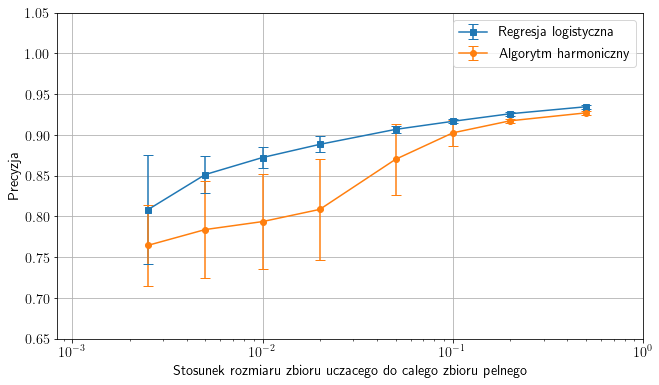
\includegraphics[width=0.95\linewidth]{img/results/wyniki-pelen.png}
	\caption{Wykres uzyskanej precyzji dla różnych rozmiarów zbioru uczącego, wykonane dla zbioru pełnego.}	\label{fig:wyniki-pelen}
\end{figure}
\par
Patrząc na wykres na rysunku \ref{fig:wyniki-pelen} w\,przypadku mniejszych zbiorów uczących widać wyraźną przewagę regresji liniowej. Używając jej, mając zaklasyfikowany nawet tylko 1\% danych, jesteśmy w\,stanie uzyskać precyzję w\,wysokości 87\%. Natomiast algorytm harmoniczny daje niższą precyzję w\,dodatku z\,ryzykiem odchylenia w\,zależności od dobranego zbioru. 
\par
Uzyskane wyniki robią wrażenie biorąc pod uwagę, że w\,omawianym tu przypadku, dzięki zastosowaniu regresji logistycznej z\,wiedzy na temat 150 postów jesteśmy w\,stanie z\,taką precyzją podać do jakich klas może należeć pozostałe ponad 15 tysięcy postów. Nie jest to jednak wynik, który można by zastosować w\,realnym systemie automatycznej klasyfikacji postów, chcąc aby był możliwie dokładny i\,pozbawiony błędów. 


